\documentclass[10pt,dvipsnames]{beamer}
\usepackage[T1]{fontenc}
\usepackage{libertinus}
\usepackage{amsmath}
\usepackage[most]{tcolorbox}

\usepackage{hyperref}
\hypersetup{
    colorlinks=true,
    linkcolor=blue,    % color of internal links
    urlcolor=blue,     % color of external URLs
    citecolor=blue     % color of citations
}

\usepackage{xcolor}  
\newcommand{\cb}[1]{{\color{CadetBlue}#1}}


\usetheme{Goettingen}
\setbeamertemplate{footline}[frame number]
\setbeamertemplate{navigation symbols}{}


\title{CSE574 Introduction to Machine Learning}
\subtitle{Machine Learning: Introduction}
\author{Jue Guo}
\institute{University at Buffalo}
\date{\today}

\begin{document}
\begin{frame}
    \titlepage
\end{frame}

\begin{frame}
    \frametitle{Outline}
    \tableofcontents
\end{frame}
\section{Logistics}
\begin{frame}{About This Course}
    \textbf{Instructor Information}
    \begin{itemize}
        \item \textbf{Instructor}: Jue Guo
        \item \textbf{Office Hr}: Monday 9:00AM -- 10:30AM
        \item \textbf{Location}: \href{https://buffalo.zoom.us/j/7673733717?pwd=TktTVXlDOGgxM3dRUC9UT21hNEdOQT09&omn=92002344719}{Zoom Link}
        \item Read piazza post \textbf{frequently}.
    \end{itemize}
    \textbf{Course Location and Time}
    \begin{itemize}
        \item \textbf{Location}: Norton 190
        \item \textbf{Time}: Monday, Wednesday, and Friday, 3:00 pm to 3:50 pm.
        \item Drop Date: 1/31/24
        \item Attendance is not mandatory, and all the course note will be \textbf{handwritten} or through \textbf{slides} in class. Course material on GitHub can be used as a guide but \textbf{not} the ultimate contents being delivered in class.
    \end{itemize}
    \textbf{Other Important Information}
    \begin{itemize}
        \item Read \href{https://piazza.com/class/lq6pes9vr0v135/post/20}{FDOC Checklist} on piazza. (25 minutes read)
    \end{itemize}

\end{frame}

\section{What is Machine Learning}
\begin{frame}{What is Machine Learning?}
    Machine Learning is a sub-field of computer science concerned with building algorithms that, to be useful, rely on a collection of \textcolor{red}{examples} of some phenomenon.
    \begin{itemize}
        \item These examples can come from nature, be handcrafted by humans, or be generated by another algorithm.
    \end{itemize}
    Machine learning can also be defined as the process of solving a practical problem by
    \begin{enumerate}
        \item gathering a dataset
        \item algorithmically building a \textcolor{red}{statistical model} based on that dataset.
    \end{enumerate}
    The statistical model is assumed to be used somehow to solve the practical problem. To save keystrokes, ``learning" and ``machine learning" are used interchangeably.
\end{frame}

\section{Types of Learning}
\begin{frame}{Types of Learning}
    Learning can be \textcolor{red}{supervised, semi-supervised, unsupervised, and reinforcement}.
\end{frame}

\subsection{Supervised Learning}
\begin{frame}{Supervised Learning}
    In \textbf{supervised learning}, the \textbf{dataset} is the collection of \textbf{labeled examples} \(\left\{\left(\mathbf{x}_{i}, y_{i}\right)\right\}_{i=1}^{N}\). Each element \(\mathbf{x}_{i}\) among \(N\) is called a \textbf{feature vector}.
    \begin{itemize}
        \item A feature vector is a vector in which each dimension \(j=1,...,D\) contains a value that describes the example somehow. That value is called a \textbf{feature} and is denoted as \(x^{(j)}\).
        \item The \textbf{label} \(y_i\) can be either an element belonging to a finite set of \textbf{classes} \{\(1,2,...,C\)\}, or a real number, or a more complex structure, like a vector, a matrix, a tree, or a graph. Unless otherwise stated, \(y_i\) is either one of a finite set of classes or a real number.
    \end{itemize}
    The goal of a \textbf{supervised learning algorithm} is to use the dataset to produce a \textbf{model} that takes a feature vector \(\mathbf{x}\) as input and outputs information that allows deducing the label for this feature vector.
\end{frame}

\subsection{Unsupervised Learning}
\begin{frame}{Unsupervised Learning}
    In \textbf{unsupervised learning}, the dataset is a collection of unlabeled examples \(\{\mathbf{x_i}\}^{N}_{i=1}\). The goal of \textbf{unsupervised learning algorithm} is to create a \textbf{model} that takes a feature vector \(\mathbf{x}\) as input and either transforms it into another vector or into a value that can be used to solve a practical problem.
    \begin{itemize}
        \item In \textbf{clustering}, the model returns the id of the cluster for each feature vector in the dataset.
        \item In \textbf{dimensionality reduction}, the output of the model is a feature vector that has fewer features than the input \(\mathbf{x}\).
        \item In \textbf{outlier detection}, the output is a real number that indicates how \(\mathbf{x}\) is different from a ``typical'' example in the dataset.
    \end{itemize}
\end{frame}

\subsection{Semi-Supervised Learning}
\begin{frame}{Semi-Supervised Learning}
    In \textbf{semi-supervised learning}, the dataset contains both labeled and unlabeled examples. Usually, the quantity of unlabeled examples is much higher than the number of labeled examples. The goal of a \textbf{semi-supervised learning algorithm} is the same as the goal of the supervised learning algorithm.
    \begin{itemize}
        \item using many unlabeled examples can help the learning algorithm to find a better model. It could look counter-intuitive that learning could benefit from adding more unlabeled examples. It seems we add more uncertainty to the problem. \textcolor{red}{However, when you add unlabeled examples, you add more information about your problem: a larger sample reflects better the probability distribution the data we labeled came from}.
    \end{itemize}
\end{frame}

\subsection{Reinforcement Learning}
\begin{frame}{Reinforcement Learning}
    \textbf{Reinforcement learning} is a subfield of machine learning where the machine ``lives" in an environment and is capable of perceiving the \textit{state} of the environment as a vector of features. The machine can execute \textit{actions} in every state. Different actions bring different \textit{rewards} and could also move the machine to another state of the environment.  The goal of a \textbf{reinforcement learning algorithm} is to learn a \textit{policy}.
    \begin{itemize}
        \item A policy is a function (similar to the model in supervised learning) that takes the feature vector of a state as input and outputs an optimal action to execute in that state. The action is optimal if it maximizes the \textit{expected average reward}.
    \end{itemize}
    Reinforcement learning solves a particular kind of problem where decision making is sequential, and the goal is long term, such as game playing, robotics, resource management, or logistics. In our class, we will \textbf{not} include reinforcement learning.
\end{frame}

\section{How Supervised Learning Works?}
\begin{frame}{How Supervised Learning Works?}
    Supervised learning is the type of machine learning most frequently used in practice. The supervised learning process starts with gathering the data. The data for supervised learning is a collection of pairs (input, output).
    \begin{itemize}
        \item \textcolor{red}{\underline{\textit{Input}}} could be anything, email messages, pictures, or sensor measurements.
        \item \textcolor{red}{\underline{\textit{outputs}}} are usually real numbers, labels (cat, dog, mouse), vectors (four coordinates), sequence or some other structure.
    \end{itemize}
\end{frame}

\subsection{Supervised Learning Example: Spam Detection}
\begin{frame}{Spam Detection: Problem Definition}
    \cb{\textbf{Problem Definition}} You gather the data, 10,000 email messages, each with a label either ``spam" or ``not\_spam". Now you have to convert each email message into a feature vector. one common way to convert a text into a feature vector, called \textbf{bag of words}
    \begin{tcolorbox}[enhanced jigsaw, breakable, pad at break*=1mm, colback=gray!20!white, colframe=black!85!black, title=\textbf{Bag of Words}]
        \textbf{Dictionary}: [``offer", ``win", ``free", ``money", ``hello", ``meeting", ``regards"]
        \begin{itemize}
            \item Email 1 (Spam): ``Win free money now!''
                  \begin{itemize}
                      \item "offer": 0, "win": 1, "free": 1, "money": 1, "hello": 0, "meeting": 0, "regards": 0

                            This becomes \([0,1,1,1,0,0,0]\)
                  \end{itemize}
            \item Email 2 (Non-Spam): ``Hello, please confirm the meeting schedule. Regards''
        \end{itemize}
    \end{tcolorbox}
    However, the Dictionary will be a lot bigger and contains 20,000 alphabetically sorted words.
\end{frame}

\subsection{Spam Detection: Learning Algorithm}
\begin{frame}{Learning Algorithm: SVM}
    Following the similar procedure, you now have machine readable input data, but the output labels are still in the form of human-readable text. Some learning algorithms require transforming labels into numbers.
    \begin{itemize}
        \item Some algorithms require numbers like 0 to represent ``not\_spam'' and 1 as ``spam''
        \item \textbf{Support Vector Machine} (SVM): positive label (``spam'') has a numeric value of +1, and the negative label (``not\_spam'') has the value of -1.
    \end{itemize}
    At this point, you have a \textbf{dataset} and a \textbf{learning algorithm}, so you are ready to apply the learning algorithm to the dataset to get the \textbf{model}.
\end{frame}

\begin{frame}
    SVM sees every feature vector as a point in a high-dimensional space (20,000-dimensional). The algorithm puts all feature vectors on an imaginary 20,000 dimensional plot and draws an imaginary 19,999-dimensional line (a \textit{hyperplane}) that separates examples with positive labels from examples with negative labels.
    \begin{itemize}
        \item In machine learning, the boundary separating the examples of different classes is called \textbf{decision boundary}.
        \item The equation of the hyperplane is given by two \textbf{parameters}, a real-valued vector \(\mathbf{w}\) of the same dimensionality as our input vector \(\mathbf{x}\), and a real number \(b\):
              \begin{equation}
                  \mathbf{w} \mathbf{x}-b=0
              \end{equation}

              where the expression wx means \(w^{(1)} x^{(1)}+w^{(2)} x^{(2)}+\ldots+w^{(D)} x^{(D)}\), and \(D\) is the number of dimensions of the feature vector \(\mathbf{x}\).
    \end{itemize}
\end{frame}

\begin{frame}
    The predicted label for some input feature vector \(\mathbf{x}\) is:
    \begin{equation}
        y=\operatorname{sign}(\mathbf{w} \mathbf{x}-b)
    \end{equation}
    where \(\operatorname{sign}\) is a mathematical operator that takes any value as input and returns +1 if the input is a positive number or -1 if the input is a negative number.
    The \textcolor{red}{goal} of the \textbf{learning algorithm} -- SVM in this case -- is to leverage the dataset and find the optimal values \(\mathbf{w}^{*}\) and \(b^{*}\). Once the learning algorithm identifies these optimal values, the \textbf{model} \(f(\mathbf{x})\) is then defined as:
    \begin{equation}
        f(\mathbf{x})=\operatorname{sign}\left(\mathbf{w}^{*} \mathbf{x}-b^{*}\right)
    \end{equation}
    Therefore, to \textcolor{red}{predict} whether an email message is spam or not spam using an SVM model,
    you have to take the text of the message, convert it into a feature vector, then multiply this
    vector by \(\mathbf{w}^{*}\), subtract \(b^{*}\) and take the sign of the result. This will give us the prediction (+1 means "spam", -1 means "not\_spam").
\end{frame}

\subsection{Optimization Problem}
\begin{frame}{Optimization Problem}
    Now, how does the machine find $\mathbf{w}^{*}$ and $b^{*}$?
    \begin{itemize}
        \item It solves an \textbf{optimization problem}. Machines are good at optimizing functions under constraints.
    \end{itemize}


    So what are the constraints we want to satisfy here?
    \begin{itemize}
        \item   First of all, we want the model to predict the labels of our 10,000 examples correctly. Remember that each example $i=1, \ldots, 10000$ is given by a pair $\left(\mathbf{x}_{i}, y_{i}\right)$, where $\mathbf{x}_{i}$ is the feature vector of example $i$ and $y_{i}$ is its label that takes values either -1 or +1 .
    \end{itemize}
    So the constraints are naturally:

    $$
        \begin{array}{ll}
            \mathbf{w} \mathbf{x}_{i}-b \geq+1 & \text { if } y_{i}=+1 \\
            \mathbf{w} \mathbf{x}_{i}-b \leq-1 & \text { if } y_{i}=-1
        \end{array}
    $$
\end{frame}

\begin{frame}
    We would also prefer that the hyperplane separates positive examples from negative ones with the largest \textbf{margin}.
    \begin{itemize}
        \item The margin is the distance between the closest examples of two classes, as defined by the decision boundary. A large margin contributes to a better generalization, that is how well the model will classify new examples in the future.
        \item  To achieve that, we need to minimize the Euclidean norm of $\mathbf{w}$ denoted by $\|\mathbf{w}\|$ and given by $\sqrt{\sum_{j=1}^{D}\left(w^{(j)}\right)^{2}}$.
    \end{itemize}


    So, the optimization problem that we want the machine to solve looks like this:
    \begin{itemize}
        \item  \textbf{\textit{Minimize $\|\mathbf{w}\|$ subject to $y_{i}\left(\mathbf{w} \mathbf{x}_{i}-b\right) \geq 1$ for $i=1, \ldots, N$.}}
    \end{itemize}


    The expression $y_{i}\left(\mathbf{w} \mathbf{x}_{i}-b\right) \geq 1$ is just a compact way to write the above two constraints. The solution of this optimization problem, given by $\mathbf{w}^{*}$ and $b^{*}$, is called the \textbf{statistical model}, or, simply, the model. The process of building the model is called \textbf{training}.
\end{frame}

\subsection{SVM: 2D Example}
\begin{frame}{SVM: 2D Example}
    For two-dimensional feature vectors, the problem and the solution can be visualized as shown in the figure.
    \begin{itemize}
        \item The blue and orange circles represent, respectively, positive and negative examples, and the line given by $\mathbf{w} \mathbf{x}-b=0$ is the decision boundary.
    \end{itemize}
    \begin{figure}[ht]
        \centering
        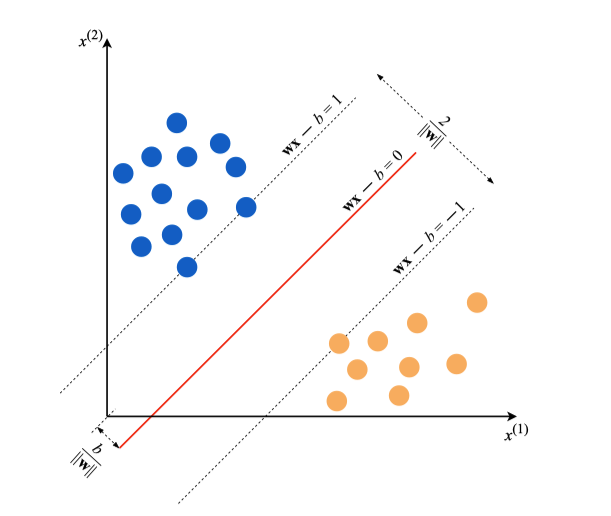
\includegraphics[width=0.5\linewidth]{imgs/intro_1.png}
        \caption{An example of an SVM model for two-dimensional feature vectors.}
    \end{figure}

\end{frame}

\begin{frame}
    Why, by minimizing the norm of $\mathbf{w}$, do we find the highest margin between the two classes?
    \begin{itemize}
        \item Geometrically, the equations $\mathbf{w} \mathbf{x}-b=1$ and $\mathbf{w} \mathbf{x}-b=-1$ define two parallel hyperplanes, as you see in figure. The distance between these hyperplanes is given by $\frac{2}{\|\mathbf{w}\|}$, so the smaller the norm $\|\mathbf{w}\|$, the larger the distance between these two hyperplanes.
    \end{itemize}
    \begin{figure}[ht]
        \centering
        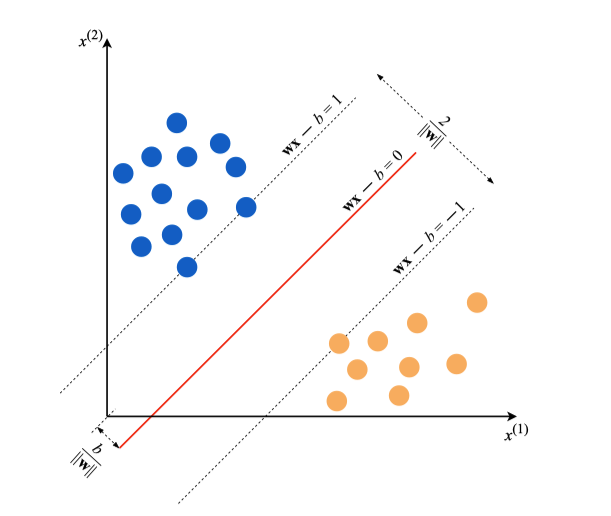
\includegraphics[width=0.5\linewidth]{imgs/intro_1.png}
        \caption{An example of an SVM model for two-dimensional feature vectors.}
    \end{figure}
\end{frame}

\subsection{Conclusion}
\begin{frame}{Conclusion}
    That's how Support Vector Machines work. This particular version of the algorithm builds the so-called linear model.
    \begin{itemize}
        \item It's called linear because the decision boundary is a straight line (or a plane, or a hyperplane). SVM can also incorporate kernels that can make the decision boundary arbitrarily non-linear.
    \end{itemize}
    In some cases, it could be impossible to perfectly separate the two groups of points because of noise in the data, errors of labeling, or \textbf{outliers} (examples very different from a "typical" example in the dataset). Another version of SVM can also incorporate a penalty hyperparameter\footnote{A hyperparameter is a property of a learning algorithm, usually (but not always) having a numerical value. That value influences the way the algorithm works. Those values aren’t learned by the algorithm itself from data. They have to be set by the data analyst before running the algorithm.} for misclassification of training examples of specific classes.
\end{frame}

\begin{frame}
    At this point, you should retain the following: \textbf{\textit{any classification learning algorithm that builds a model implicitly or explicitly creates a decision boundary.}}
    \begin{itemize}
        \item  The decision boundary can be straight, or curved, or it can have a complex form, or it can be a superposition of some geometrical figures.
        \item The form of the decision boundary determines the \textbf{accuracy} of the model (that is the ratio of examples whose labels are predicted correctly).
        \item The form of the decision boundary, the way it is algorithmically or mathematically computed based on the training data, differentiates one learning algorithm from another.
    \end{itemize}
    In practice, there are two other essential differentiators of learning algorithms to consider: \textcolor{red}{speed of model building and prediction processing time}. In many practical cases, you would prefer a learning algorithm that builds a less accurate model quickly. Additionally, you might prefer a less accurate model that is much quicker at making predictions.
\end{frame}

\section{Why the Model Works on New Data?}
\begin{frame}{Why the Model Works on New Data?}
    Why is a machine-learned model capable of predicting correctly the labels of new, previously unseen examples?
    \begin{itemize}
        \item If two classes are separable from one another by a decision boundary, then, obviously, examples that belong to each class are located in two different subspaces which the decision boundary creates.
    \end{itemize}
    \begin{figure}[ht]
        \centering
        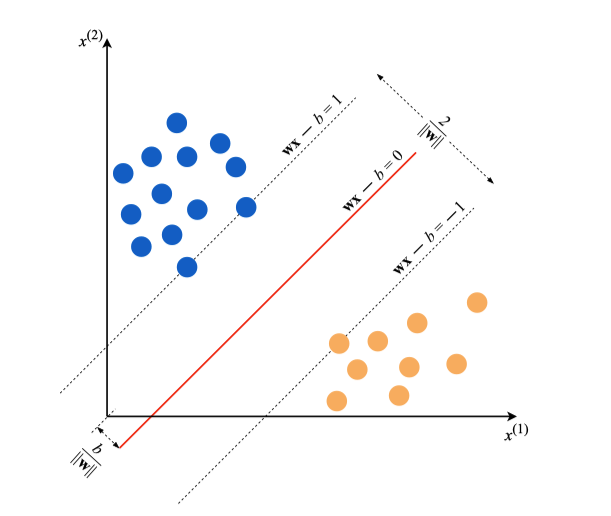
\includegraphics[width=0.5\linewidth]{imgs/intro_1.png}
        \caption{An example of an SVM model for two-dimensional feature vectors.}
    \end{figure}
\end{frame}

\begin{frame}
    If the examples used for training were selected randomly, independently of one another, and following the same procedure, then, statistically, it is \textit{more likely} that the new negative example will be located on the plot somewhere not too far from other negative examples.
    \begin{itemize}
        \item The same concerns the new positive example: it will \textit{likely} come from the surroundings of other positive examples.
    \end{itemize}
    In such a case, our decision boundary will still, with \textit{high probability}, separate well new positive and negative examples from one another.
    \begin{itemize}
        \item For other, \textit{less likely} situations, our model will make errors, but because such situations are less likely, the number of errors will likely be smaller than the number of correct predictions.
    \end{itemize}
    Intuitively, the larger is the set of training examples, the more unlikely that the new examples will be dissimilar to (and lie on the plot far from) the examples used for training.
    \begin{itemize}
        \item To \textcolor{red}{minimize the probability of making errors on new examples}, the SVM algorithm, by looking for the largest margin, explicitly tries to draw the decision boundary in such a way that it lies as far as possible from examples of both classes.
    \end{itemize}
\end{frame}

\begin{frame}
    \begin{center}
        \Huge Questions?
    \end{center}
\end{frame}
\end{document}